% Samlar lite saker här som vi eventuellt vill ha med i appendixet, alternativt ta bort helt.

% Heat map E.coli #1
\textcolor{blue}{Should this be in the discussion?}\\
By creating a heat map of the Poisson distances between the \textit{E. coli} samples, the relation between the six studied samples could be verified. The heat map is presented in figure \ref{fig:E.coli_pois} and shows two clear clusters that group case samples in one cluster and control samples in the other cluster.  \textcolor{blue}{This was as expected.} The colour intensity increases as the distance decreases, which indicates a higher resemblance between samples. \textcolor{blue}{Poisson distances were used instead of Euclidean distances, since/because ...}

\begin{figure}[ht]
    \centering
    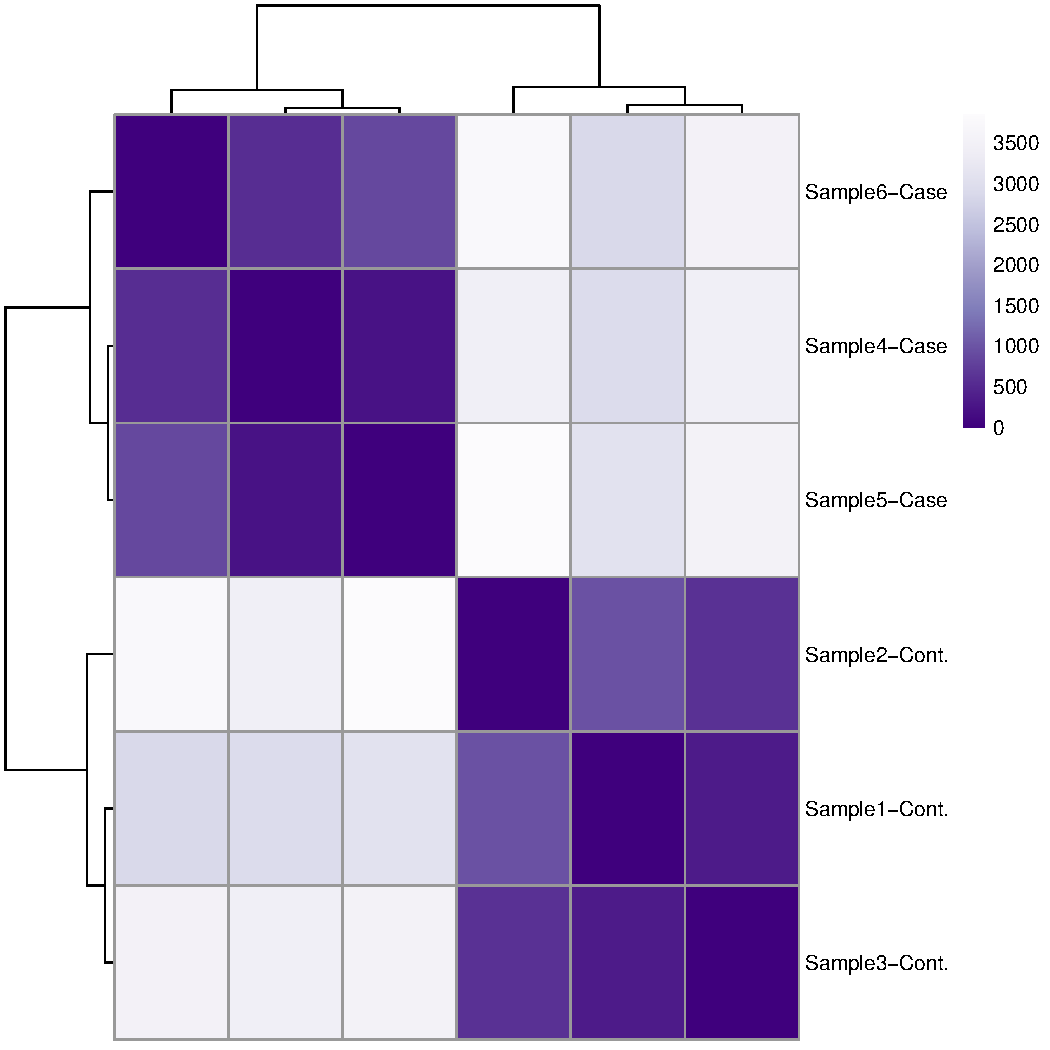
\includegraphics[scale=0.6]{Figures/Pois_dist_heat_E_coli.pdf}
    \caption{The Poisson distances between \textit{E. coli} samples visualised by colour intensity. Samples are clustered according to resemblance.}
    \label{fig:E.coli_pois}
\end{figure}
 
 % Histogram E.coli #3or4
The p-values obtained from the differential expression analysis of \textit{E. coli} are plotted in a histogram in figure \ref{fig:E.coli_hist}. The distribution is approximately uniform for p-values $>$ 0.05. \textcolor{blue}{This is good since the assumption is that p-values are uniformly distributed under the null hypothesis and that they are $<$ 0.05 when the null hypothesis is rejected.}

\begin{figure}[h!]
    \centering
    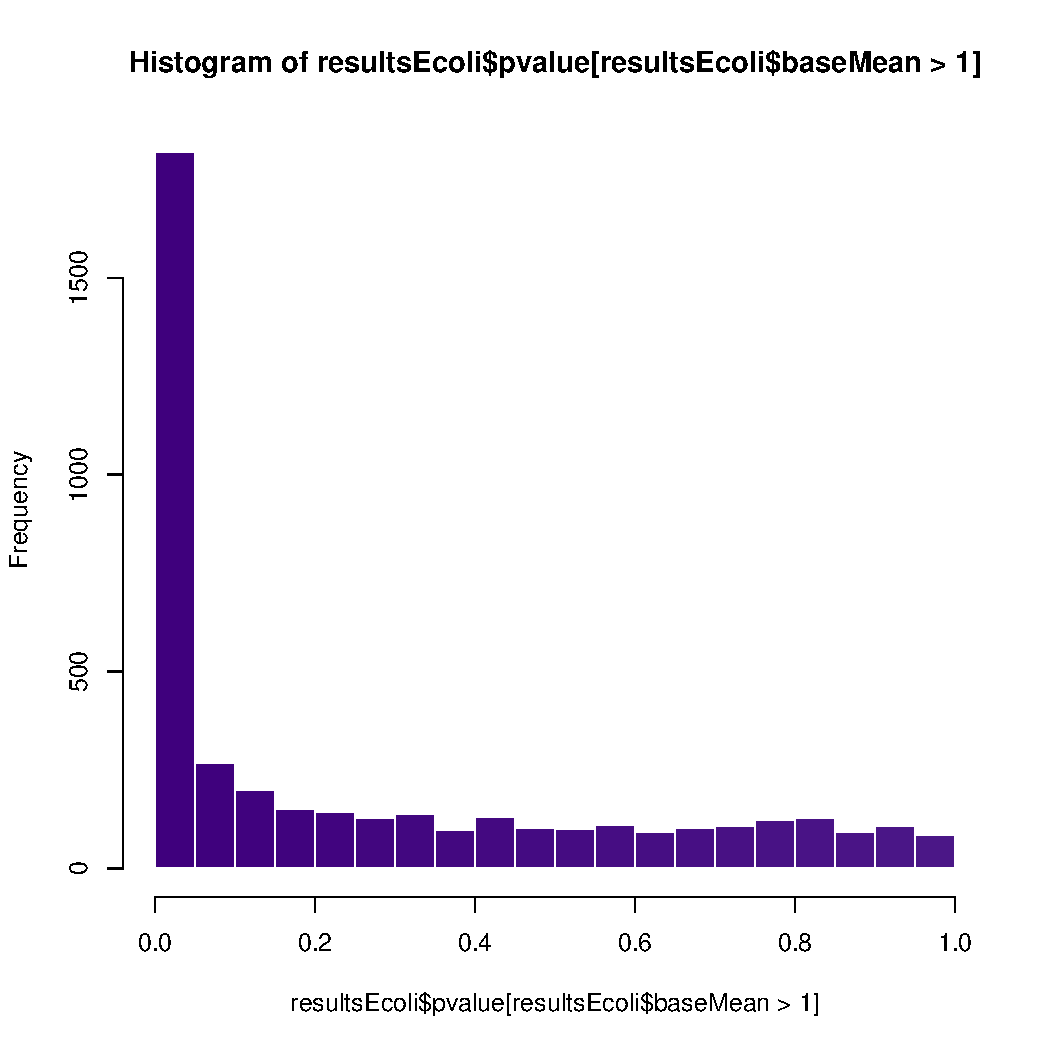
\includegraphics[scale=0.5]{Figures/Histogram_pvalues_E_coli.pdf}
    \caption{The histogram of p-values obtained for genes expressed in \textit{E. coli}. The distribution is approximately uniform for p-values $>$ 0.05. }
    \label{fig:E.coli_hist}
\end{figure}

% heat map plasmid #1
The heat map created for Poisson distances between the plasmid samples is presented in figure \ref{fig:plasmid_hist} and shows a clear cluster which groups the control samples together. The case samples are also grouped together, although their Poisson distances is larger, as seen in the figure by the lighter colour. This indicates that they are less similar than the control samples. \textcolor{blue}{The heat map was as expected. Compared to the heat map created for the \textit{E. coli} samples, this heat map shows larger resemblance between all samples and less defined clusters, which could be due to lower gene expression for the plasmid and thus fewer gene counts in the samples.}
\begin{figure}[h!]
    \centering
    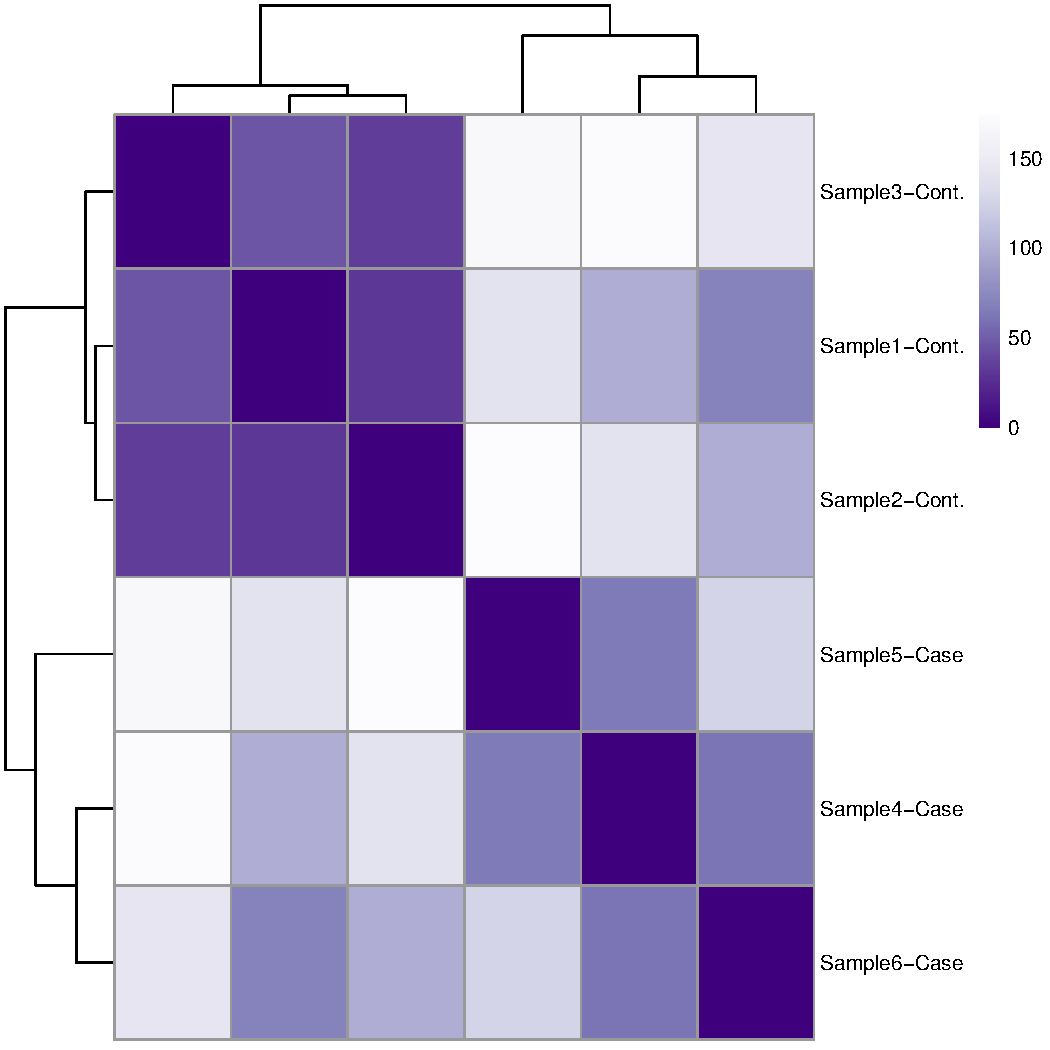
\includegraphics[scale=0.6]{Figures/Pois_dist_heat_plasmid.pdf}
    \caption{The Poisson distances between plasmid samples visualised by colour intensity. Samples are clustered according to resemblance.}
    \label{fig:plasmid_pois}
\end{figure}

% Histogram plasmid #3or4
The p-values obtained from the differential expression analysis of the plasmid are plotted in a histogram in figure \ref{fig:plasmid_hist}. The distribution is roughly uniform for p-values $>$ 0.05. 
\begin{figure}[h!]
    \centering
    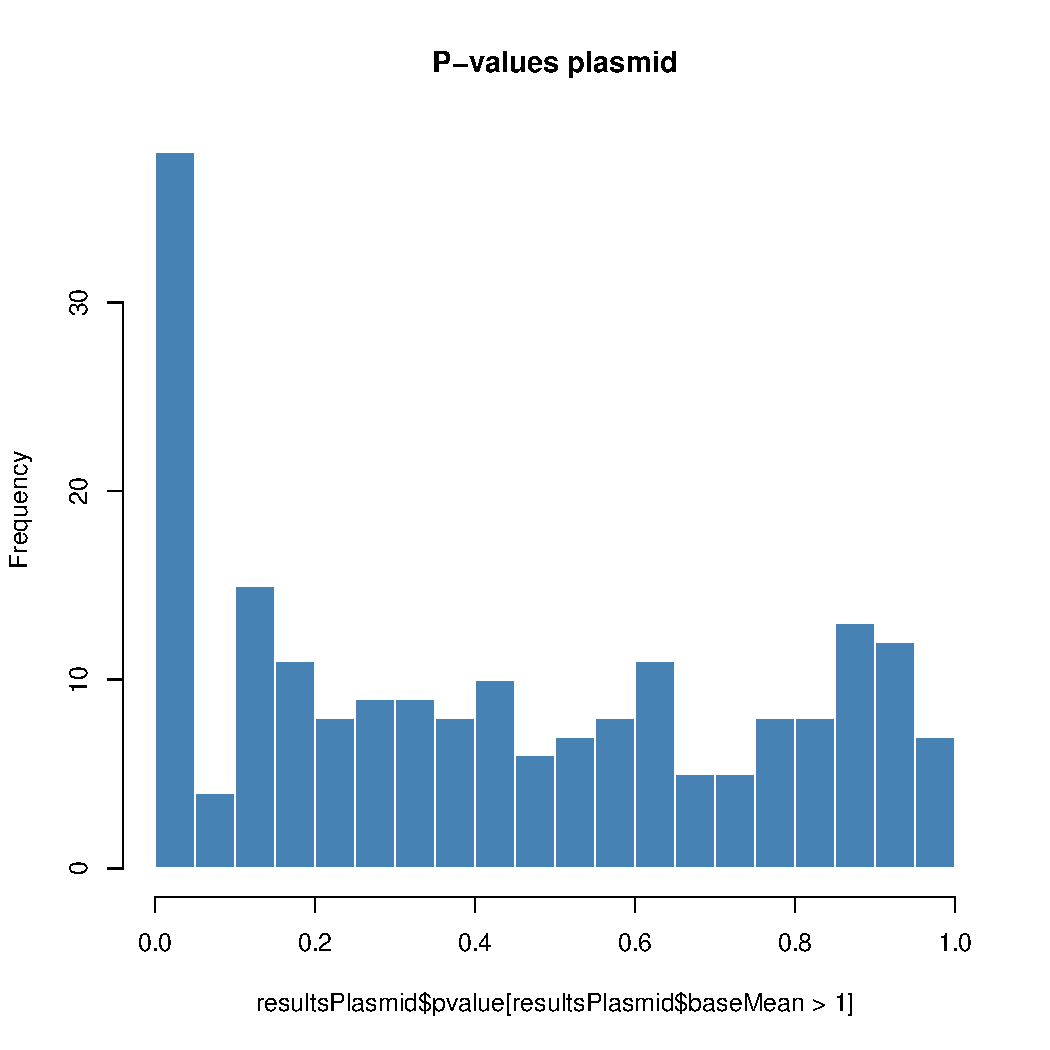
\includegraphics[scale=0.5]{Figures/Histogram_pvalues_plasmid.pdf}
    \caption{The histogram of p-values obtained for genes expressed in the plasmid. The distribution is roughly uniform for p-values $>$ 0.05.}
    \label{fig:plasmid_hist}
\end{figure}
